% -*- root: ../../main.tex -*-
\section{Interazioni}
\label{sec:interactions_design}

\subsubsection{Interazione tra Engine, ECS e controller}
Come spiegato nel \ref{sec:ecs_design}, i vari gestori di componenti che compongono l'ECS sono coordinati tra di loro tramite un coordinator. Esso fa da punto di contatto con l'engine vero e proprio esponendo il metodo \textbf{updateAllSystems}, che corrisponde a un tick del gioco. Esso viene incapsulato nel metodo \textbf{update} esposto dall' interfaccia \textbf{UpdateableEngine}, implementata dal \textbf{GameEngine}. In questo modo è possibile per il \textbf{GameLoop} interagire con l'engine, esponendo solo lo stretto necessario.
Quando il gioco viene eseguito in modalità singleplayer il controller si occupa di creare l'engine e di attaccarci il mediator, mentre al join di una partita multiplayer esso verrà detachato e verrà creato l'attore client. Invece, durante l'hosting di una partita multiplayer il server si affianca al gamescreen e tramite il mediator riceve gli eventi dall'engine e li comunica ai client partecipanti alla partita.
\begin{figure}[H]
	\centering
	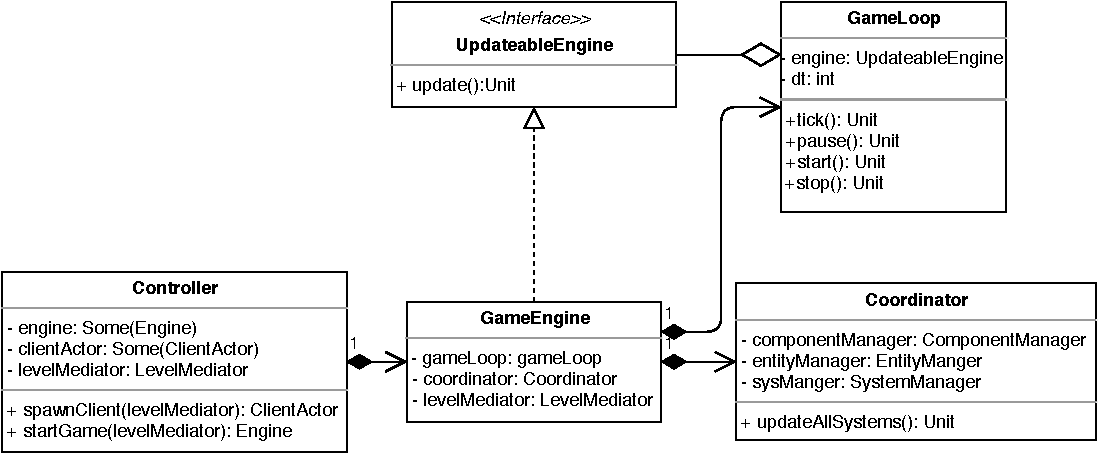
\includegraphics[width=\columnwidth]{drawio/ECS-engine-controller/ecs-engine-controller.pdf}
	\caption{Diagramma raffigurante ecs, engine e controller e le loro interazioni.}
	\label{fig:ecs-engine-controller}
\end{figure}



\subsubsection{Interazione tra Controller e View}
Per renedere possibile l'aggiornamento della View da parte del controller è stato utilizzato il pattern observer, fornendo al controller un oggetto che implementa il trait \textbf{ObserverUI}. Esso fornisce al controller quattro metodi per poter comandare la view: 
\begin{itemize}
    \item updateSettings: ;
    \item updateLobbyStatus: mostra nella view il nuovo status della lobby, quando si unisce un nuovo giocatore alla partita, o al cambiamento dello stato di "ready" di un giocatore;
    \item updateClientLobbySettings: aggiorna i client sui cambiamenti delle impostazioni globali della partita effettuati lato server; 
    \item gameStartedByServer: causa il caricamento del GameScreen, chiamato nel client alla ricezione del messaggio di avvio dal server;
\end{itemize}



Invece, per garantire la possibilità alla view di comunicare al controller le operazioni necessarie al setup delle differenti modalità di gioco gli viene fornito il trait \textbf{UpdatableUI}, implementato dal controller, che espone i seguenti metodi:
\begin{itemize}
    \item attacheUI, detacheUI: servono per registrare e de-registrare (nel caso venga fatto eseguire il gioco in modalità server "headless") la view tra gli observer del controller;
    \item modifySettings, loadStats: consentono di caricare e modificare le statistiche e le impostazioni salvate su file;
    \item selectClientMode, selectServerMode, selectSinglePlayer: permettono lo switch tra le varie modalità di gioco, e causano il setup o la distruzione dei vari componenti;
    \item joinServerLobby, modifyMatchSetup: metodi relativi all'interazione con la lobby in modalità multiplayer;
    \item startGame: in modalità singleplayer e in modalità multiplayer quando si è host, notifica al controller l'intenzione dell'utente di iniziare una partita;
\end{itemize}




\begin{figure}[H]
	\centering
	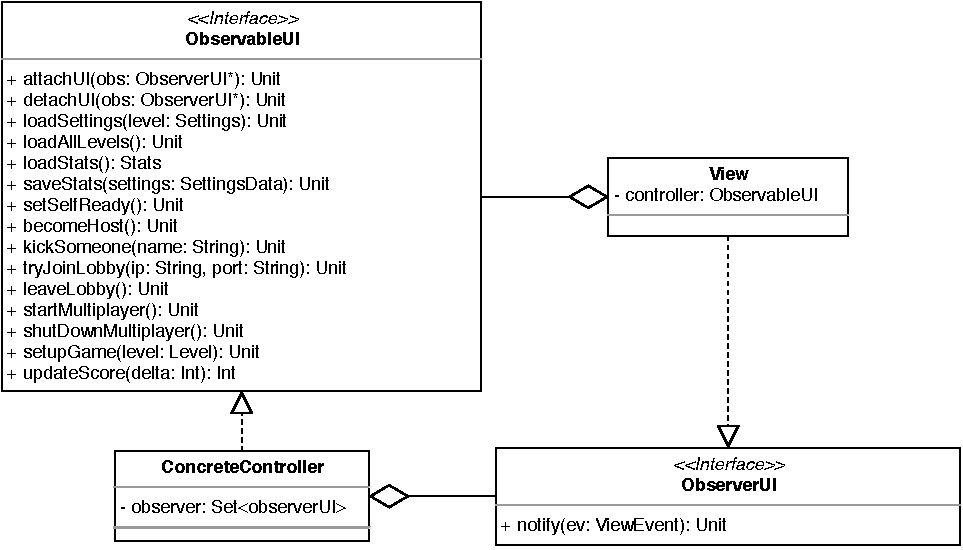
\includegraphics[width=\columnwidth]{drawio/view-controller-observer/view-controller-observer.pdf}
	\caption{Diagramma raffigurante view, controller e observer e le loro interazioni.}
	\label{fig:view-controller-observer}
\end{figure}